\documentclass{article}

\usepackage[utf8]{inputenc}
\usepackage{fixltx2e}
\usepackage{graphicx} 
\usepackage[a4paper, total={6in, 8in}]{geometry}
\usepackage{enumitem}
\usepackage{float}

\author{Marc Juvillà Garcia}
\title{\vspace{-2cm}Homework 2. Machine Learning (MIIS)}

\begin{document}
\maketitle
Consider a simplified learning scenario. Assume that the input dimension is
one. Assume that the input variable x is uniformly distributed in the interval
[-1, 1]. The data set consists of 2 points \{x\textsubscript{1} , x\textsubscript{2}\} and assume that the target
function is f (x) = x\textsuperscript{2} . Thus, the full data set is D = \{(x\textsubscript{1}, x\textsubscript{1}\textsuperscript{2}), (x\textsubscript{2}, x\textsubscript{2}\textsuperscript{2})\}. The
learning algorithm returns the line fitting these two points as g (H consists of
functions of the form h(x) = ax + b). We are interested in the test performance
(E\textsubscript{out}) of our learning system with respect to the squared error measure, the
bias and the variance.

\begin{enumerate}[label=(\alph*)]
\item Give the analytic expression for the average function $\bar{g}$(x).

Hypothesis g\textsuperscript{D}(x), where D = \{(x\textsubscript{1}, x\textsubscript{1}\textsuperscript{2}), (x\textsubscript{2}, x\textsubscript{2}\textsuperscript{2})\}:
\begin{equation} 
g\textsuperscript{D}(x) = \left(\frac{x\textsubscript{2}\textsuperscript{2} - x\textsubscript{1}\textsuperscript{2}}{x\textsubscript{2} - x\textsubscript{1}}\right)(x - x\textsubscript{1}) + x\textsubscript{1}\textsuperscript{2}
\end{equation}
Which leads to:
\begin{equation} 
g\textsuperscript{D}(x) = (x\textsubscript{1} + x\textsubscript{2})x - x\textsubscript{1}x\textsubscript{2}
\end{equation}

$\bar{g}$(x) is defined as:
\begin{equation} 
\bar{g}(x) = E\textsubscript{D}[g\textsuperscript{D}(x)]
\end{equation}
Then, computing the expectation for all the possible datasets:
\begin{equation} 
\bar{g}(x) = \frac{1}{2} \int_{-1}^{1} \frac{1}{2} \int_{-1}^{1} g\textsuperscript{D}(x) \,dx\textsubscript{1}\,dx\textsubscript{2} = \frac{1}{4} \int_{-1}^{1} \int_{-1}^{1} (x\textsubscript{1} + x\textsubscript{2})x - x\textsubscript{1}x\textsubscript{2} \,dx\textsubscript{1}\,dx\textsubscript{2} = 
\frac{1}{4} \int_{-1}^{1} 2x\textsubscript{1}x \,dx\textsubscript{1} = 0
\end{equation} 

\item Describe an experiment that you could run to determine (numerically)
$\bar{g}$(x), E\textsubscript{out}, bias, and var.

We could determine experimentally these parameters by running a large amount of linear regression trainings. In each iteration, we would:
\begin{enumerate}
\item Generate a dataset D = \{(x\textsubscript{1}, x\textsubscript{1}\textsuperscript{2}), (x\textsubscript{2}, x\textsubscript{2}\textsuperscript{2})\} with random x\textsubscript{1} and x\textsubscript{2} and a large dataset D\textsubscript{val} = \{(x\textsubscript{1}, x\textsubscript{1}\textsuperscript{2}) ... (x\textsubscript{N}, x\textsubscript{N}\textsuperscript{2})\}.
\item Train g\textsuperscript{D}(x)
\item Compute the error of g\textsuperscript{D}(x) with D\textsubscript{val}.
\end{enumerate}

After all the iterations are finished, we can obtain E\textsubscript{out} by taking the mean for all the linear regression errors.\\
$\bar{g}$(x) can be obtained by computing the mean of all the weights for each g\textsuperscript{D}(x).\\
Bias can be obtained by computing the error of $\bar{g}$(x).\\
Variance can be computed taking the squared difference between the output of each g\textsuperscript{D}(x) and $\bar{g}$(x).

\item Run your experiment and report the results. Compare E\textsubscript{out} with bias+var.
Provide a plot of your $\bar{g}$(x) and f(x) (on the same plot).

For the experiments, I computed 10.000 g\textsuperscript{D}(x) and generated a D\textsubscript{val} of 1.000 samples for each iteration. The results are the following:

$E\textsubscript{out} = 0.5341$\\
$bias = 0.2027$\\
$variance = 0.3356$\\
$bias + variance = 0.5384$\\

As expected, $E\textsubscript{out}\approx bias+variance$

\begin{figure}[H]
    \centering
	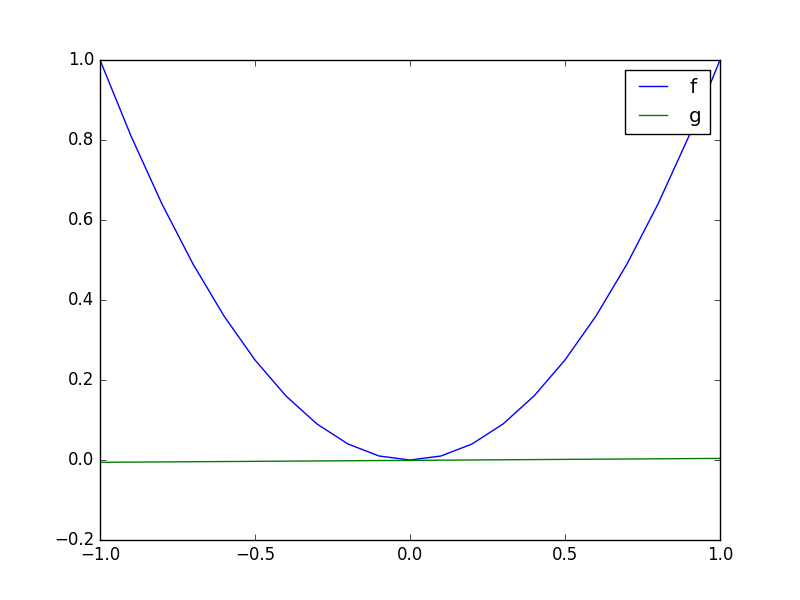
\includegraphics[scale=0.35]{images/3.png} 
    \caption{Comparison between $f(x)$ and $\bar{g}$(x).}
\end{figure}

\item Compute analytically what E\textsubscript{out}, bias, and var should be.

E\textsubscript{out}:
\begin{equation}
E\textsubscript{out} = E\textsubscript{D}[E\textsubscript{out}(g\textsuperscript{D})] = E\textsubscript{D}[E\textsubscript{x}[(g\textsuperscript{D}(x) - f(x))^2]]
\end{equation}

Combining (2), (5) and $f(x) = x^2$, we get:
\[
E\textsubscript{out} = \frac{1}{8} \int_{-1}^{1} \int_{-1}^{1} \int_{-1}^{1} (g\textsuperscript{D}(x) - f(x))^2 \,dx\,dx\textsubscript{1}\,dx\textsubscript{2} = \frac{8}{15} \approx 0.5333
\]
bias:
\begin{equation}
bias = E\textsubscript{x}[(\bar{g}(x) - f(x))^2] = E\textsubscript{x}[(\bar{g}(x) - f(x))^2]
\end{equation}

Knowing (4) and $f(x) = x^2$:
\[
bias = E\textsubscript{x}[f(x)^2] = \frac{1}{2} \int_{-1}^{1} x^4 \,dx = \frac{1}{5} \approx 0.2
\]

variance:
\begin{equation}
variance = E\textsubscript{x}[E\textsubscript{D}[(g\textsuperscript{D}(x) - \bar{g}(x))^2]]
\end{equation}

Knowing (2) and (4):
\[
variance = E\textsubscript{x}[E\textsubscript{D}[g\textsuperscript{D}(x)^2]] = \frac{1}{8} \int_{-1}^{1} \int_{-1}^{1} \int_{-1}^{1} ((x\textsubscript{1} + x\textsubscript{2})x - x\textsubscript{1}x\textsubscript{2})^2 \,dx\,dx\textsubscript{1}\,dx\textsubscript{2} = \frac{1}{3} \approx 0.333
\]

As we can see, the results are almost identical to the ones obtained in the experiment. The small differences can be blamed to the fact that, as we can see in Figure 1, the experimental $\bar{g}$(x) is not 0 (as computed analytically), but has a small slope and a small bias.

\end{enumerate}
\end{document}
